\chapter{Survey}
\label{chp:amtsurvey} 

\section{Constructing the Survey}

\subsection{How and why we chose this design}
%hvorfor vi satte spørsmålene der vi gjorde osv osv. Design!
%Hvorfor surveymonkey?
%hvordan vi gikk fram på AMT? hvorfor amt?

\section{Survey Results}
%Hvor mange svar vi fikk og sånn
%hvor lenge den lå ute på amt
%Hvordan vi har gått gjennom resultatene, hva vi har fokusert på og hvorfor!

\begin{figure}[h!]
\centering
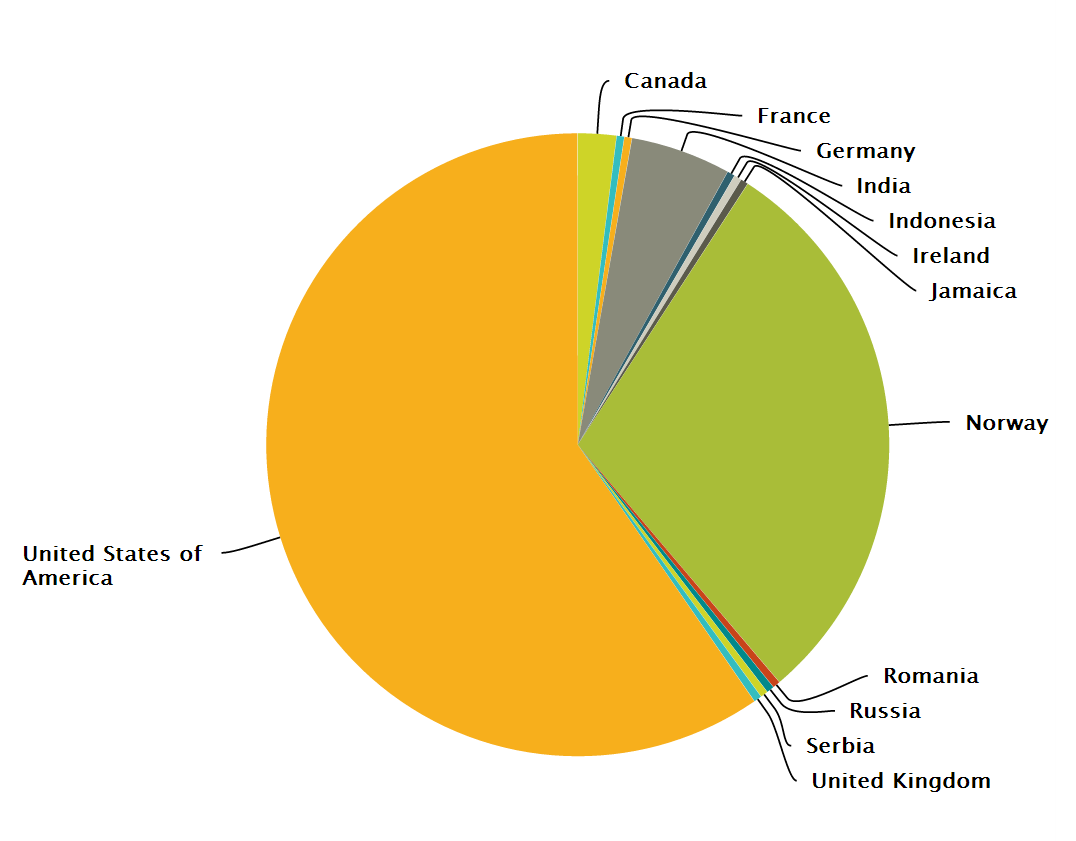
\includegraphics[width=1\textwidth]{land.png}
\caption[Distribution of the participant's country of origin]{\textbf{Distribution of the participant's country of origin.} This graph shows the distribution of the participant's country of origin. Most of the participants are from the United Stated of America and Norway.} 
\label{fig:land}
\end{figure}

\subsection{Demographics}

\begin{figure}[h!]
\centering
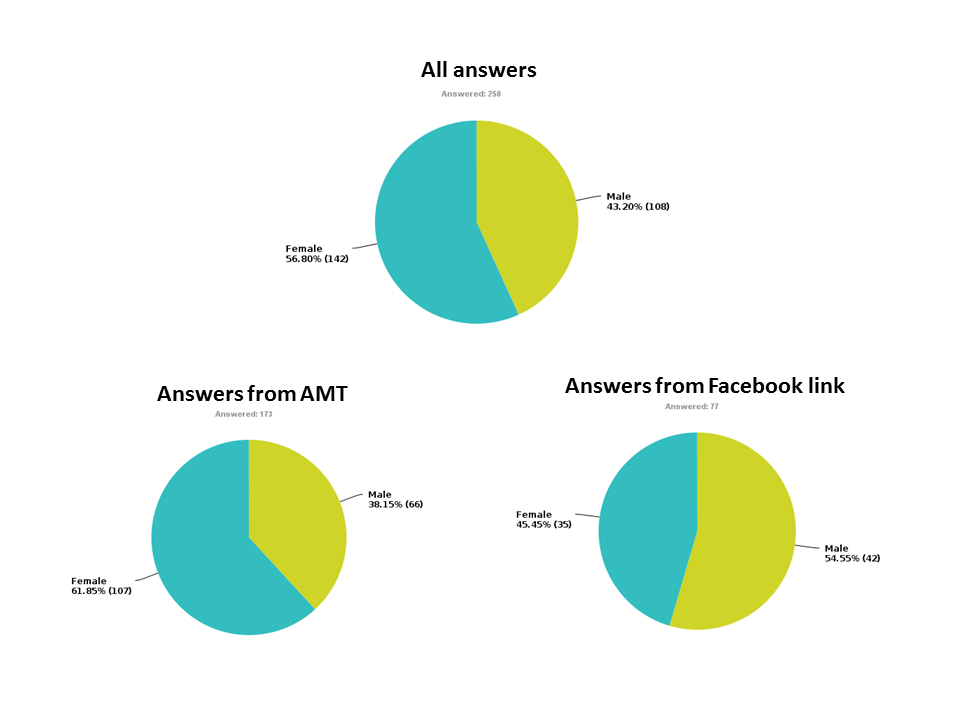
\includegraphics[width=1\textwidth]{gender.png}
\caption[Gender distribution]{\textbf{Gender distribution}. This graph shows the overall gender distribution (on the top), gender distribution from AMT (to the left) and the gender distribution from the Facebook link (to the right).} 
\label{fig:gender}
\end{figure}

As mentioned before we distributed our survey on two platforms; Amazon Mechanical Turk (AMT) and Facebook. As you can see in \fref{fig:land}, the distribution was mainly divided between two countries, the United States of America and Norway. Other countries are also represented; Canada, France, Germany, India, Indonesia, Ireland, Jamaica, Romania, Russia, Serbia and United Kingdom. 77 of the 250 responses were collected through the Facebook link, and out of these 77 people 96\% (74 people) are from Norway. 173 of the 250 respondents took the survey via Amazon Mechanical Turk, and out of these people 85,5\% (148 people) are from the United Stated of America. 

\paragraph{}
The majority of the total respondents were female. They accounted for 56,80\% of the responses, which is 142 responses. This means that 43,20\% of the total respondents were male, with a 108 responses. We saw a difference in the gender distribution from the Facebook link and from AMT. On AMT 38,15\% were men, and 56,80\% were female. On Facebook 54,55\% were male, and 45,55\% were female. In other word the majority of respondents on AMT were females, in contrary to Facebook, were the majority of respondents were men. The different gender distributions are shown in the \fref{fig:gender}.
 
\paragraph{}
Among the participants the age ranged betweetn 19 and 76. The average age is 31. The average age of the AMT participants (33 years old) are higher than the average age of the Facebook participants (27 years old). When we look at the total income of the household per year and employment status, we find a wide range of variety among the participants. We have several participants in each group of income. Although the majority of the participants are employed for wages or students, all of the other employment status' are represented. This is consistent with former studies of AMT users \cite{incentivesAmt}. 


\subsection{Frequency in Checking Facebook Privacy Settings}

\subsubsection{Never Checked Facebook Privacy Settings During the Last Year}

\begin{figure}[h!]
\centering
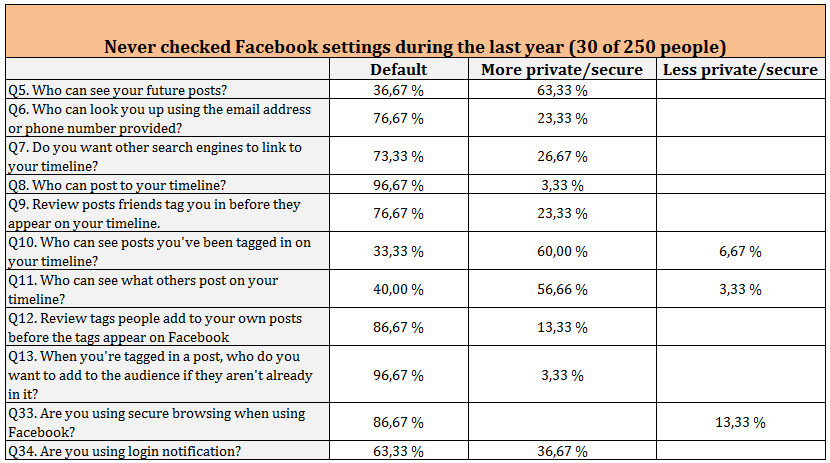
\includegraphics[width=1\textwidth]{nevercheckedtable.png}
\caption[Never checked Facebook privacy settings during the last year]{\textbf{Never checked Facebook privacy settings during the last year.} Forklare hva figuren viser.} 
\label{fig:neverchecked}
\end{figure}

30 of the people who answered our survey stated that they have never checked their privacy settings during the last year. Even though they have not checked the privacy settings during the last year, most of them have done some changes to their settings before the previous year. The reason for this assumption is that their settings differ from the default settings.  
The average number of friends for the people who have never checked Facebook privacy settings during the last year is 162, and their average age is 39. 

In \fref{fig:neverchecked} you can see a percentage distribution over Facebook settings among the people who have never checked their Facebook privacy settings during the last year. We have divided them into tree categories; "Default", "More secure", and "Less secure". You end up under the category "Default" if your settings is similar to the default settings anno 2013. See section \ref{subsec:default2013} for more detailed description of the default settings on Facebook. You end up under the "More secure" category if you have changed the default setting to a more secure settings. The "Less secure" is for those who have made changes to their settings which is less secure than the default settings. 

The majority of these users are active users, since 67\% of them checks their Facebook page at least once a day. 

60\% of the people who had never checked their Facebook privacy settings during the last year \textit{did not} consider changing their privacy settings after reviewing them. 40\% of them wanted to make their privacy settings more private. 

We have a quote from a 67 year old woman that took our survey (with Ph.D and only 5 Facebook friends) that emphasised many user's unawareness when it comes to different Facebook settings: "Now you have scared me. I am alone and afraid".


\subsubsection{Checks Facebook Privacy Settings "Once a month" or "Once a week or more"}

\begin{figure}[h!]
\centering
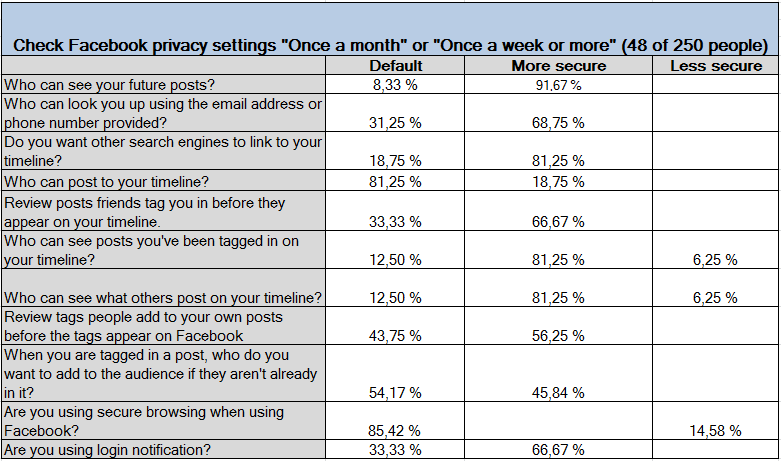
\includegraphics[width=1\textwidth]{checkonceaweekormoretable.png}
\caption[Checks Facebook privacy settings "Once a month" or "Once a week or more"]{\textbf{Checks Facebook privacy settings "Once a month" or "Once a week or more".} Forklare figuren mer nøye her} 
\label{fig:onceaweekormore}
\end{figure}

48 of the people who answered our survey stated that they check their privacy settings "Once a month" or "Once a week or more". The average number of friends for these people is 416, and their average age is 28,5. 

In \fref{fig:onceaweekormore} you can see a percentage distribution of what kind of settings the people who check their privacy settings "Once a month" or "Once a week or more" have. We have divided them into the same categories as above; "Default", "More secure", and "Less secure".  

85\% of the people who checked their Facebook privacy settings "Once a month" or "Once a week or more" during the last year, has checked their Facebook page at least once a day during the last month. This indicates that the majority of those who check their settings frequently are also very active Facebook users. 

70,83\% of these people did not consider changing privacy settings after reviewing them. 27,08 \% wanted to make their privacy settings more private, and 2,08\% considered changing them to more public. 


%12 of the 48 people in this category answered yes on the question whether or not facebook had affected their personal life negativally. Half of these had situations with friends posting unwanted pictures (av forskjellige grunner) of them.

%One guy: Two accounts; one under a pseudonym for friends only and on with strict settings for the rest of the world. "Privacy is important to me. It is meaningless not to give others the same courtesy" - Random guy with 420 friends that are 43 years old. 

\subsubsection{Comparing the ones Who Have Never Checked their Facebook Privacy Settings During the Last Year and the Ones Who Checks "Once a month" or "Once a week or more"} 

\paragraph{Activity level}
The majority of both groups checks their Facebook page at least once a day. The percentage is a little bit higher for the people who have checked their privacy settings "Once a month" or "Once a week or more" during the last year. 85\% of them checks their Faceook page at least once a day, in contrast to the other group (who have never checked their settings during the last year) with 67\% checking their Facebook page at least once a day. This indicates that the ones who have never checked their settings during the last year does not refrain from doing this because they are inactive users. One assumption for this may be that the users are unaware of the settings. 40\% of them stated that they wanted to make their settings more private after taking the survey. This backs up the assumption about unawareness.  

\paragraph{More secure settings for those who check their settings more often?}
As \fref{fig:neverchecked} and \fref{fig:onceaweekormore} shows, the people who checks their facebook settings frequently have changed their settings to more secure to a higher degree. 
%FYLL INN MER HER

\paragraph{Considered changing settings}
The percentage of those wanting to make their settings more private is higher for those who have never checked settings during the last year with 40\% of the group. Only 27\% of the frequent setting-checkers wanted to make their settings more private. 
None of the people who have never checked their settings during the last year wanted to make their settings more public, unlike the other group (those who check "Once a month" or "Once a week or more") where 2\% actually considered changing them to more public. Overall the frequent settings-checkers were more pleased with their settings than the once who had never checked them during the last year. 70\% of the frequent settings-checkers did not consider changing their settings after reviewing them. Although the ones who have never checked their settings during the last year have far less secure settings than the other group, 60\% of them did not consider changing their settings either. 


\subsection{Interdependent Privacy}



